\documentclass[9pt,24pt,twocolumn]{article}
\usepackage[utf8]{inputenc}
\usepackage[spanish]{babel}
\usepackage{amsmath}
\usepackage{amsfonts}
\usepackage{amssymb}
\usepackage{graphicx}
\usepackage[left=1.5cm,right=1.5cm,top=1.5cm,bottom=2.4cm]{geometry}
\author{Caro Diaz Juan, Correa Barcos Valentina, Restrepo Aguilera Yulissa
\\
\\
\textit{Facultad de Ingeniería, Universidad Tecnológica de Bolívar}
\\
{\textit{Cartagena, Bolívar}}
\\
\\{\small {juandiaz7289@gmail.com}}
\\{\small {valencorreabarco@hotmail.com}}
\\{\small {yulissatatiana@gmail.com}}
}

\date {}
{\title{{\Huge ENCRIPTACIÓN Y DESENCRIPTACIÓN DE DATOS}}}

\begin{document}

\maketitle

\emph{Resumen— El cifrado es el proceso de ocultar datos o archivos mediante el uso de una clave o contraseña que consigue que, quienes accedan a ellos sin la contraseña adecuada, no puedan encontrar ninguna utilidad en los mismos, puesto que resulta difícil descifrar su contenido. Un problema común de seguridad a todos los sistemas de computo es el evitar que personas no autorizadas tengan acceso  al   sistema, ya   sea  para  obtener   información, efectuar cambios en una porción o en la totalidad de la base de datos. Se presentan mecanismos para garantizar la seguridad y aplicación de uno de ellos.}
\\

\begin{center}
{I. INTRODUCCIÓN}
\end{center}

{Es necesario, crear diferentes mecanismos, dirigidos a garantizar la confidencialidad y autenticidad de los documentos electrónicos, todo ello es parte de una nueva tecnología denominada Criptografía. Se aborda el tema de la seguridad informática en una base de datos diseñada en MySQL.}
\\

{Los datos críticos pueden ser solo un pequeño porcentaje de toda la información que la empresa almacena, pero es la más valiosa. Y todo elementos o datos prioritarios se deben vigilar y rastrear para el bien de la empresa o compañía.}
\\

{Este artículo consiste en el proceso de encriptación y desencriptación de los datos críticos que se encuentran en una base de datos realizada en MySQL.}
\\

\begin{center}
{II. CRIPTOGRAFIA}
\end{center}

{El uso de la encriptación o también llamado criptografía se usa desde la Antigua Grecia. Es del griego de donde viene el nombre de la ciencia del cifrado, la criptografía: krypto “ocultar” y graphos “escribir”, es decir escritura oculta.}
\\

{La encriptación es un conjunto de técnicas que tratan sobre la protección de la información frente a observadores no autorizados, ocultando datos o archivos mediante el uso de una clave. Ha sido usada a través de los años para mandar mensajes confidenciales con el propósito que sólo las personas autorizadas puedan entenderlos. A este proceso de “esconder” y poder recibir el archivo “escondido” se llama encriptación y desencriptación respectivamente.}
\\

{Pero la confidencialidad no es lo único que permite la criptografía. También resuelve otros problemas de seguridad, como certificar la autenticidad e integridad (chequear que la información transmitida no ha sido modificada) de la información.}
\\

{Actualmente la criptografía ha evolucionado hacia sistemas mucho más complicados de romper y se usa a diario para aplicaciones diversas como conexiones seguras a ciertas páginas de Internet a las que se envía información sensible, almacenamiento de datos seguro, o firma electrónica.}
\\

{Como finalidad de la criptografía es poder garantizar el secreto entre la comunicación de dos remitentes, ya sea, personas u organizaciones, y además asegurar que la información que se envía sea real y confiable de dos maneras, que el remitente sea realmente quien dice ser y que el contenido del mensaje enviado, llamado criptograma, no haya sido modificado en su tránsito.}
\\

{En esta rama de la seguridad informática podemos definir el uso en su historia, siendo la criptografía muy antigua como lo es la escritura, pero ha tomado más fuerza hoy en día con sus aplicaciones en sistemas informáticos y los nuevos algoritmos de cifrado de la información asegurando así los pilares fundamentales sobre los que se basa la criptografía:}
\\

{-	Seguridad: asegurarse que el texto del mensaje solo pueda ser leído por el destinatario.}
\\

{-	Integridad: certeza que el mensaje no ha sufrido ninguna manipulación posterior de los datos.}
\\

{-	Autenticidad: certeza del remitente, acredita quien es su autor.}
\\

{Las claves usadas para el cifrado son combinaciones de símbolos, que pueden ser letras, números, signos de puntuación, etc. Por lo tanto, la seguridad está expuesta a posibles ataques en el momento de compartir los datos. Para evitar esto se debe tener en cuenta las siguientes reglas:}
\\

{a) Claves con gran longitud, necesitando mas recursos para cubrir todo el rango rápidamente y llegar a la clave.}
\\

{b)  Cambio regular de nuestra clave.}
\\

{c) Utilizar varios tipos de caracteres, para que sea aún mucho más difícil de adivinar.}
\\

{d)  No utilizar palabras de diccionario o nombres propios.}
\\

{Finalmente, entre las limitaciones de la criptografía está el hecho que este método tiende a degradarse con el tiempo, en donde los algoritmos se hacen más fáciles de quebrar debido al avance de la velocidad y potencia de los equipos de computación. Estos algoritmos criptográficos son vulnerables a los ataques de fuerza bruta (forzar a encontrar la clave de cifrado), la cual es más fácil de aplicar a medida que avanza el tiempo.}
\\

\begin{center}
{III. SEGURIDAD DE UNA BASE DE DATOS}
\end{center}

{La seguridad de la información en una base de datos, implica proteger los datos de operaciones y accesos que pongan en riesgo la existencia, consistencia e integridad de los datos.
Esto se logra mediante mecanismos que permiten desde el código de la aplicación controlar el acceso y los roles de usuarios. Todo algoritmo o método de encriptación tiene la función de codificar los datos para dificultar su lectura y que sea indescifrable.}
\\


\textit{A. AES (Advanced Encryption Standard):}

{El uso de la encriptación AES en MySQL es la más segura que se ha incorporado al gestor de base de datos, utiliza dos funciones: AES\_ENCRYPT y AES\_DECRYPT, para utilizar en forma directa en sentencias SQL.}

{AES es rápido, fácil de implementar por código, por lo que este método se convierte en un estándar de cifrado, se está utilizando actualmente en muchos sistemas a gran escala y sitios en web.}
\\

\textit{B. Base64:}

{La encriptación Base64 se basa en caracteres ASCII, se utiliza para codificar información en correos electrónico, enviar información en una red normalmente se utiliza para encriptar datos que no son texto, imágenes, archivos adjuntos, etc.}
\\

\textit{C. MD5 (Message Digest 5):}

{El método de criptografía MD5 o Resumen del Mensaje 5 es un algoritmo de reducción criptográfico de 128 bits muy utilizado para cifrar contraseñas como Wordpress, Prestashop, Joomla entre otros.}

{No se puede decodificar, aunque algunas webs van recolectando palabras y convirtiéndolas a MD5 para tener una base de datos con posibles codificaciones.}
\\


\begin{center}
{IV.  PROBLEMÁTICA}
\end{center}

{El avance tecnológico de hoy en día nos facilita tanto las comunicaciones entre nosotros como la manipulación e intercambio de información para compartir información en recursos tecnológicos, centralizar determinados procesos y abaratar costes en prestación de servicios por las empresas. Estos avances permiten que los datos personales circulen de manera rápida y sean almacenados indefinidamente en algún lugar.}
\\

{El flujo de datos personales no solo influye auxiliar respecto de empresas, entidades o personas que utilizan o realizan diversas actividades con la información como por ejemplo apartar un tiquete de avión o comprar en Internet, pero estas no se han realizado sin costes de poner en peligro la vida privada de las personas. Para nadie es secreto que, sin demasiadas técnicas, la información puede ser objeto de un tratamiento ilícito, por lo que, sería una transferencia de datos sin consentimiento del propietario de dicha información violando sus derechos fundamentales constitucionalmente protegidos. De ahí la aparición de diversos modos de que estos ciber-ataques en la información sean dados.}
\\

{Con estos posibles ataques de robo de información que existen tanto en la red como fuera de ella, se hace de manera necesaria que cada empresa o compañía cuente con un equipo de seguridad informática para garantizar la seguridad en sus datos críticos y/o confidenciales. Siendo el cifrado de datos uno de las mejores soluciones para este tipo de problemas, donde para poder ver esta información requiere de una clave que solo conocen pocas personas.}
\\

{En una empresa, que maneja información de algunos de sus usuarios, como correo y número de sus respectivas tarjetas de crédito, todo esto almacenado en una base de datos en MySQL, requiere transferir esta información a otro líder, por vía web, y para evitar robo de la información privada que tienen de los usuarios se le hace necesario encriptar esta información con una clave que solo conocerá la persona a la cual se le enviará la información. Ahora procederemos a ver como se realiza la encriptación de estos datos.}
\\

\begin{center}
{V.  SOLUCIÓN}
\end{center}

{La criptografía es fundamental cuando nos referimos a la seguridad, esto nos ayudara a mantener la información segura, además también se ha utilizado con fines delictivos, el propósito de este proyecto es saber el proceso que se requiere para poder encriptar información o datos que se encuentran en una base de datos en MySQL. Se utilizará el método de seguridad AES, que además de ser la mas segura, ya se encuentra incorporada en MySQL Workbench.}

\begin{figure}[h]
\begin{flushleft}
    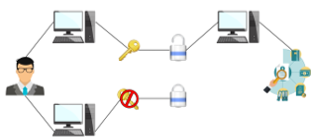
\includegraphics{bas9}
\end{flushleft}
{\tiny \caption{Diagrama de la estructura a utilizar}}
  \label{fig:10}
\end{figure}

{Utilizando las funciones de encriptar (AES\_ENCRYPT) y desencriptar (AES\_DECRYPT) ya incorporadas.  Tendremos una base de datos con información de una empresa, en este caso los datos a utilizar serán un id que representara al usuario, nombre del usuario, correo y su respectivo número de tarjeta de crédito y así para los diferentes trabajadores de la empresa. Luego de crear y haber llenado la tabla a la cual encriptaremos, así:}

\begin{figure}[h]
\begin{flushleft}
    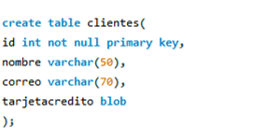
\includegraphics{bas1}
\end{flushleft}
{\tiny \caption{Creación de tabla clientes}}
  \label{fig:1}
\end{figure}

\begin{figure}[h]
\begin{flushleft}
    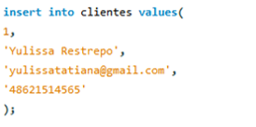
\includegraphics{bas2}
\end{flushleft}
\caption{Insertar datos a la tabla clientes}
  \label{fig:2}
\end{figure}

{Tener cuenta que este proceso de insertar datos a la tabla “clientes” se realizara para cada usuario a ingresar con sus respectivos datos, en este ejemplo se insertara 15 usuarios, cada uno con sus respectivos datos.}
\\

{Ya ingresado todos los usuarios a la tabla con la sintaxis anterior se procede a ver la tabla que se observa a continuación:}

\begin{figure}[h]
\begin{flushleft}
    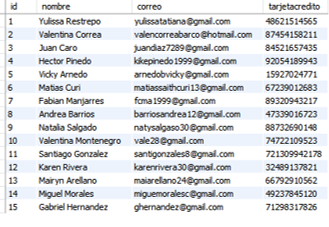
\includegraphics{bas3}
\end{flushleft}
  \caption{Tabla clientes}
  \label{fig:3}
\end{figure}

{Como es bien sabido, el numero de tarjeta de crédito de una persona es algo privado, por lo que al momento de pasar esta información a otro servidor u otro encargado de la información se recomienda que este oculto o en otras palabras, encriptado. Esto se realizara con la siguiente función, la cual recibe dos parámetros, el dato a cifrar y la clave que nosotros definimos, retorna un valor tipo blob.}

\begin{figure}[h]
\begin{flushleft}
    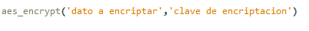
\includegraphics{bas4}
\end{flushleft}
  \caption{Función de encriptación de datos}
  \label{fig:4}
\end{figure}

{Procedemos a encriptar todos los números de tarjeta con una contraseña que le vamos a poner a cada usuario, la cual será la misma, para que el proceso de desencriptación se realice en toda la columna.} 

\begin{figure}[h]
\begin{flushleft}
    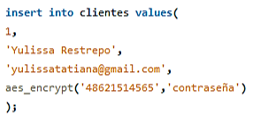
\includegraphics{bas5}
\end{flushleft}
  \caption{Aplicación de la función de encriptación}
  \label{fig:5}
\end{figure}

{Y así se realizara para cada usuario registrado en nuestra base de datos, como podemos ver la clave de cifrado es “contraseña”, la cual se utilizará mas adelante para el proceso de descifrado.}
\\

{Luego en la tabla ya cifrada, si alguien quiere acceder a los datos de la tabla no podrá conocer el valor real almacenado (en este caso) en la columna “tarjetacredito” debido a que lo ciframos anteriormente.}

\begin{figure}[h]
\begin{flushleft}
    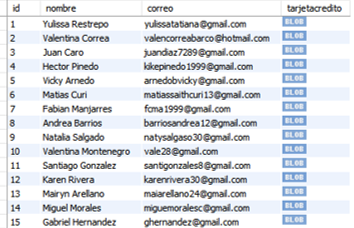
\includegraphics{bas6}
\end{flushleft}
  \caption{Tabla clientes con datos cifrados}
  \label{fig:6}
\end{figure}

{Y como ya hemos mencionado anteriormente se necesita una contraseña para volver a tener los datos encriptados, esta contraseña se especifico anteriormente. Luego de que los datos se encuentren en su lugar de destino se procederá a hacer el desencriptado de la información, con la siguiente función:}
\begin{figure}[h]
\begin{flushleft}
    
\includegraphics{bas7}
      \caption{Función de desencriptación de datos}
  \label{fig:7}
\end{flushleft}
\end{figure}

{Donde claramente necesitamos conocer la clave de cifrado. En la siguiente línea se pedirá mostrar la tabla y hacer la desencriptación ingresado la clave de cifrado:}

\begin{figure}[h]
\begin{flushleft}
    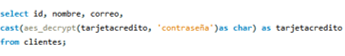
\includegraphics{bas8}
\end{flushleft}
  \caption{Aplicación de la función de desencriptación}
  \label{fig:8}
\end{figure}

{Luego de todo el proceso de desencriptación realizado anteriormente realizado podemos observar que la tabla tiene nuevamente todos los datos visibles, incluyendo el anteriormente encriptado "tarjetacredito":}

\begin{figure}[h]
\begin{flushleft}
    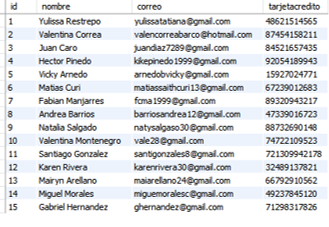
\includegraphics{bas3}
\end{flushleft}
\caption{Tabla clientes}
  \label{fig:9}
\end{figure}

\begin{center}
{VI. CONCLUSIÓN}
\end{center}

{En conclusión, la criptografía es uno de los métodos para poder proteger la información, donde vuelve completamente ilegibles los datos de un archivo y de esa manera volverlo prácticamente inservible para un usuario no autorizado a
leerlo, ya que si no cuenta con una contraseña de acceso no podrá verlo y mucho menos manipularlo. Hace parte
de la seguridad informática donde hay diferentes métodos para proteger esta información como cifrado simétrico y
asimétrico. La criptografía además es muy utilizada en el ámbito laboral, donde empresas la usan para proteger sus
datos o archivos críticos y/o confidenciales.}
\\
{En este proyecto investigativo luego de analizar la seguridad en una base de datos, se realizó un ejemplo donde se aplicó el método de cifrado en una base datos realizada en MySQL. Donde ya viene incorporado funciones de cifrado y descifrado de la información en nuestra base de datos. Donde ocultaba dicha información y solo se podía acceder a ella con la clave de cifrado establecida.}
\\

{Y así comprobar la eficiencia de la criptografía para ocultar y proteger nuestros datos de personas no autorizadas
para acceder a nuestra información privada.}

\begin{center}
{REFERENCIAS}
\end{center}

{[1] Domínguez, J. (2015). Principios Básicos de Seguridad en Bases de Datos. Universidad Politécnica Territorial del Estado Aragua. [Online]. Available: }
{https://www.researchgate.net/publication/279983428
\_Principios\_Basicos\_de\_Seguridad\_en\_Bases\_de\_Datos}
\\

{[2] Marrero, Y. (2003). La Criptografía como elemento de la seguridad informática. ACIMED, 11(6). [Online]. Available: }
{http://scielo.sld.cu/scielo.php\?script\=sci\_arttext\&pid\=S1024\-94352003000600012\&lng\=es\&tlng\=es}
\\

{[3] MySQL 5.0 Manual. (2010). Funciones de encriptación. [Online]. Available: }
{http://download.nust.na/pub6/mysql/doc/refman/5.0/es
/encryption\-functions.html}
\\

{[4] Gutierrez, D. (2009). Seguridad en BD. Universidad de los Andes Venezuela. [Online]. Available: }
{http://www.codecompiling.net/files/slides/BD\_clase\_12}
{\_seguridad.pdf}
\\

{[5] Torres, W. (2018). MODELOS DE ENCRIPTACIÓN EN BASE DE DATOS MS-SQL SERVER. UNIVERSIDAD NACIONAL ABIERTA Y A DISTANCIA UNAD. [Online]. Available: }
{https://stadium.unad.edu.co/preview/UNAD.php\?url\=}
{/bitstream/10596/21344/1/79865131.pdf}
\\

{[6] Labodía, J. Protección de la infromación a través del cifrado. ACCA. [Online]. Available: }
{https://www.acta.es/medios/articulos/ergonomia\_y}
{\_seguridad/016033.pdf}

\end{document}